% Options here are passed to the article class.
% Most common options: 10pt, 11pt, 12pt
\documentclass[10pt]{datasheet}

% Input encoding and typographical rules for English language
\usepackage[utf8]{inputenc}
\usepackage[english]{babel}
\usepackage[english]{isodate}

% tikz is used to draw images in this example, but you can
% also use \includegraphics{}.
\usepackage{graphicx}
\usepackage{float}
\usepackage{subcaption}

% These define global texts that are used in headers and titles.
\title{AC01: Box Color Swapper}
\author{Basil}
\tags{autocrafting, box-color}
\date{25 December 2024}
\revision{Revision 1}
\begin{document}
\maketitle

\section{Features}

\begin{itemize}
\item{Safety features: Dry fire proof and checks if dyes are present}
\item{No idle hoppercarts}
\item{Fully hopperlocked}
\item{Small and compact}
\end{itemize}

\section{Applications}

\begin{itemize}
\item{Recoloring shulker boxes before sending them to storage}
\end{itemize}

\section{General Description}
The AC01 Box Color Swapper is a device that recolors shulker boxes using color dyes and a crafter. The device's item to color map is set using the built-in encoder. The device is designed to be safe, with features that prevent dry firing and ensure that the dyes are present. Without the necessary dyes, the device will not recolor the box. See the corresponding  \href{https://www.youtube.com/watch?v=nnvas8g5LmQ}{explanation video on Youtube}. Inspired by Obi's encoder design.
\vfill\break

\begin{figure}[H]
    \centering
    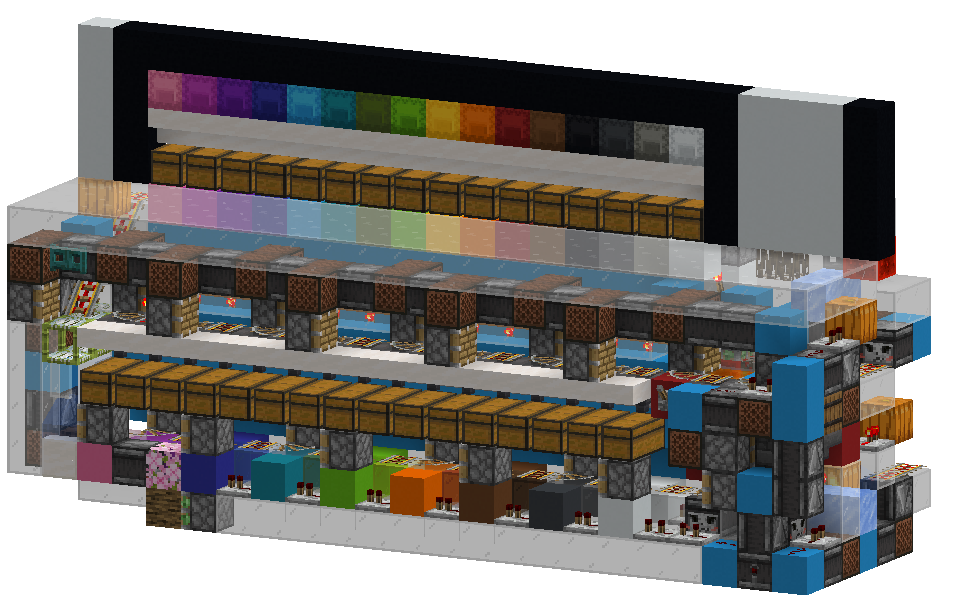
\includegraphics[width=0.48\textwidth]{area_render_30_.png}
    \caption{\centering Box Color Swapper}
\end{figure}

% For wide tables, a single column layout is better. It can be switched
% page-by-page.
\onecolumn

\section{Device Specifications}

\begin{table}[H]
    \caption{Inputs}
    \begin{tabularx}{\textwidth}{l | c | X}
        \thickhline
        \textbf{Name} & \textbf{Range} & \textbf{Description} \\
        \hline
        Box input & Box & To be recolored shulker box containing 
        items. Barrel input. \\
        \hline
        Dye input & Item & Dye items to recolor the box. 16 variants. \\
        \thickhline
\end{tabularx}
\end{table}

\begin{table}[H]
    \caption{Outputs}
    \begin{tabularx}{\textwidth}{l | c | X}
        \thickhline
        \textbf{Name} & \textbf{Range} & \textbf{Description} \\
        \hline
        Colored box & Box & Recolored shulker box with the same items as input. Waterstream output. \\
        \thickhline
\end{tabularx}
\end{table}

\begin{table}[H]
    \caption{Device Specifications}
    \begin{tabularx}{\textwidth}{l | c c c | c | X}
        \thickhline
        \textbf{Parameter} & \textbf{Min.} & \textbf{Typ.} & \textbf{Max.} &
        \textbf{Unit} & \textbf{Conditions} \\
        \hline
        Throughput  & - & 125 & - & gt & Normal Usage \\
        \hline
        Latency    & - & 120 & - & gt & From input to crafter activation. \\
        \hline
        MC Version & 1.21 & 1.21.4 & - & MCV & Latest version at time of writing: 1.21.4\\
        \hline
        Dimensions & & 23 x 12 x 7 & & Blocks & \\
        \thickhline
\end{tabularx}
\end{table}
\section{Testing Data}
\begin{table}[H]
\caption{Executed Tests}
\begin{tabularx}{\textwidth}{l | X}
    \thickhline
    \textbf{Test} & \textbf{Result} \\
    \hline
    Throughput test & Device was able to correctly recolor boxes with multiple boxes input simultaneously \\
    \thickhline
\end{tabularx}
\end{table}

\section{Download Information}
\begin{table}[H]
    \caption{Download Information}
    \begin{tabularx}{\textwidth}{l | l | l | X}
        \thickhline
        \textbf{Identifier} & \textbf{MC} & \textbf{File} & \textbf{Description} \\
        \hline
        AC01 & 1.21 & \href{https://github.com/Soontech-Annals/Archive/blob/8413f90a054b6c415703bae02badeba7541344f6/Archive/autocrafting/AC01\%20Box\%20Color\%20Swapper/AC01\_Box\_Color\_Swapper.litematic?raw=1}{AC01\_Box\_Color\_Swapper.litematic} & Schematic of device. \\
        \hline
        \thickhline
    \end{tabularx}
\end{table}

\end{document}

